\section{Linear Regression}
$y_i = \beta_1 x_{i1}+...+\beta_p x_{ip} + \epsilon_i$ ($x_{i1}\equiv 1$, so $\beta_1$ is intercept) $Y = X\beta + \epsilon$ $\epsilon_1,...,\epsilon_n$ are indep., $\mathbb{E}(\epsilon_1)=0, \text{Var} (\epsilon_i)=\sigma^2$ (homoscedastic)\\
\textbf{Least square solution}
$\hat \beta = \text{argmin}_\beta ||Y-Xb||_2^2 = (X^\top X)^{-1}X^\top Y \sim \mathcal{N}_p(\beta, \sigma^2 (X^\top X)^{-1})$ \\
$RSS=||Y-X\hat \beta||_2^2\qquad\hat \sigma^2 \approx \frac 1 {n-p}RSS$.
If $\epsilon \sim \mathcal{N}$ then: $\hat Y \sim \mathcal{N}_n(X\beta, \sigma^2 P)$,
$\mathbf{r} \sim \mathcal{N}_n(0, \sigma^2(I-P))$,
$\hat \sigma^2 \sim {\sigma^2 }/{(n-p)}\cdot \chi_{n-p}$
where $P=X(X^\top X)^{-1}X^\top $

\textbf{Interpreting R-output: }
\underline{Residuals}: Difference between what the model predicted and the actual value of y. Can be calculated as: \texttt{summary(y-model\$fitted.values)}\\
\underline{Coefficients}: the weights that minimize the sum of squared errors.\\
\underline{Std. Error} = Residual Standard Error / sqrt(sum(square(particular x variable))). \underline{t value}: Estimate / Std. Error

\begin{codebox}{r}{Linear Regression}
fit <- lm(y~x1+x2) # Fit only x1 and x2 (so p=3)
predict(fit, pred.data.frame)
# Manual fit
X <- cbind(1, x1, x2) # p = 3
XtX.inv <- solve(t(X) %*% X)
beta.hat <- XtX.inv %*% t(X.int) %*% y
res <- y - X.int %*% beta.hat # Residuals
RSE <- sqrt(sum(res^2)/(n-p)) # Residual std. error. Est. of the sd of the noise in the linear model
se.x1 <- RSE * sqrt(XtX.inv[2, 2]) # Std. error of x1
t.val.x1 <- beta.hat[2] / se.x1 # T value of x1
p.val.x1 <- 2*pt(abs(t.val.x1), df=n-p, lower=F)
# Alternative t-value
coef <- summary(fit1)$coefficients
t1 <- coef["x1","Estimate"]/coef["x1","Std. Error"]
# Poly regression
lm(wage~poly(age,4)) # Orthogonal polynomials
lm(wage~poly(age, 4, raw=T)) # Monomial basis
lm(wage~age+I(age^2)+I(age^3)+I(age^4)) # Alternative
\end{codebox}

\subsection{Tests and model selection}
\textbf{Entry-wise test}\\
$H_0: y = X\beta + \epsilon$ with $\beta_j=0$
$H_A: y = X\beta + \epsilon$ with $\beta_j\neq 0$\\
Under $H_0: \frac{\hat \beta_j - (E[\hat \beta_j]=0)}{\sqrt{\sigma^2(X^\top X)^{-1}_{jj}}} \sim \mathcal{N}(0,1)$
t-statistic: $\frac{\hat \beta_j}{\sqrt{\hat \sigma^2 (X^\top X)^{-1}_{jj}}} \sim t_{n-p}$\\
\textbf{P-Value:} P(obs. a value of the test stat. that is as extreme or more extreme than the one we saw if $H_0$ is true).
If $< \alpha$ then reject $H_0$.
\textbf{ANOVA (Analysis of variance)}\\
$\Vert Y-\bar Y \Vert^2=\Vert  \hat Y - \bar Y\Vert^2+\Vert Y-\hat Y\Vert^2$\\
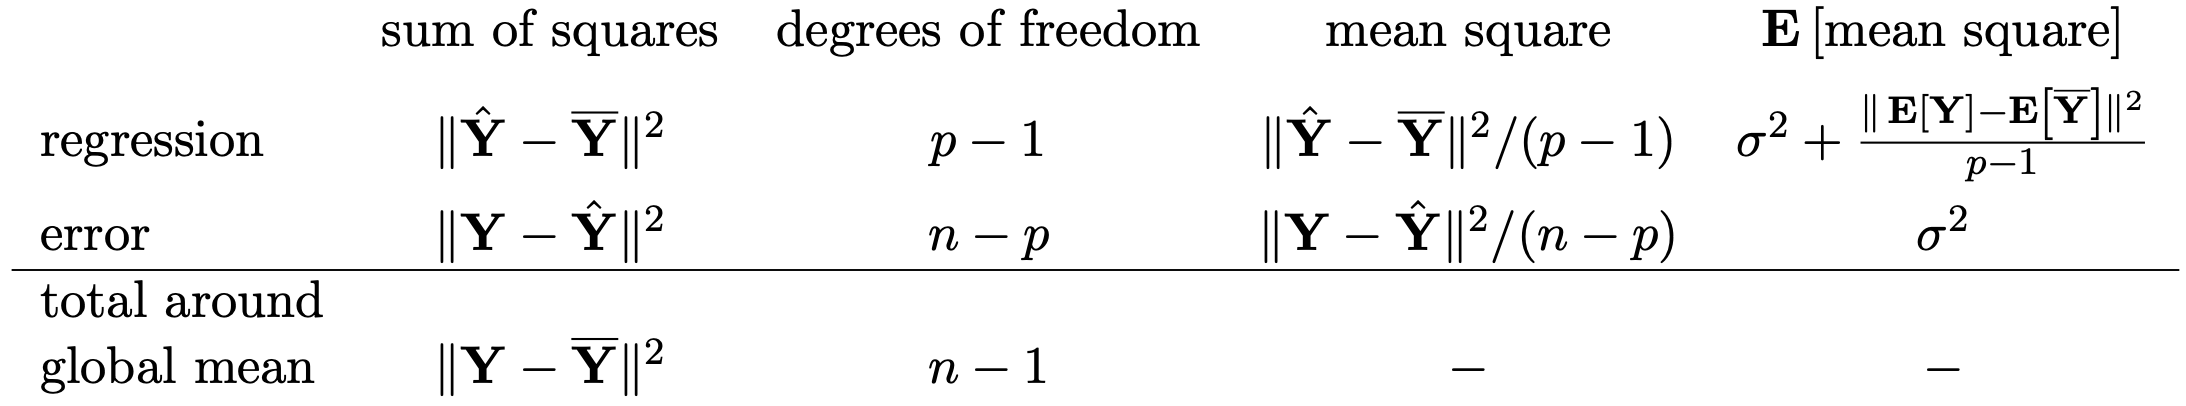
\includegraphics[width = 7cm]{ANOVA.png}
Under the null hypothesis $H_0:\beta = 0$ We have that:\\
$F=\frac{\Vert  \hat Y - \bar Y\Vert^2/(p-1)}{\Vert Y-\hat Y\Vert^2/(n-p)}\sim F_{p-1,n-p}$\\

\begin{codebox}{r}{P-Values \& ANOVA}
fit.smaller <- lm(y ~ x1)
# Anova uses RSS and DoF of largest (last) model, so
# use ascending order!
anova(fit.smaller, fit, fit.all)
# Overall F-Test
fit.empty <- lm(y ~ 1, data=...) # Empty model
anova(fit.empty, fit) # Compare models
# Alternative F-test
Ftest <- summary(fit)$fstatistic
pval <- 1 - pf(Ftest[1], df1=Ftest[2], df2=Ftest[3])
\end{codebox}


\textbf{R\textsuperscript{2} (Coefficient of determination):} the proportion of the total variation of the response $Y$ around its mean $\bar{Y}$ that is explained by the regression $\hat{Y}$ (via the ANalysis Of VAriance decomposition)
$R^2=\frac{||\hat{Y}-\bar{Y}||^2}{||Y-\bar{Y}||^2}=1-\frac{||Y-\hat{Y}||^2}{||Y-\bar{Y}||^2} = \frac{ESS}{TSS} = 1-\frac{RSS}{TSS}$

\begin{codebox}{r}{R squared}
RSE <- sqrt(sum(residuals(fit)^2)/(n-p))
RSS <- sum(res^2) # Residual sum of squares
TSS <- sum((y - mean(y))^2) # Total sum of squares
R.sq <- 1 - RSS / TSS
AdjR2 <- 1 - (RSS/(n-p))/(TSS/(n-1))
\end{codebox}

\subsection{Model selection}
To penalize large model we use Mallows statistic.\\
$C_P(\mathcal{M}) = n^{-1} RSS(\mathcal{M}) - \hat \sigma ^2 + 2n^{-1} \hat\sigma ^2\vert M\vert$. We can simply chose among all submodels the one with the best $C_p$ score, or, if it's too hard\\
\textbf{Forward stepwise:} 1) Fit $M_0$ 2) For $k=0,...,p-1$ fit all $p-k$ models with 1 additional predictor and select best (smallest RSS): $M_k$. 3) Select best among $M_0,....,M_p$ using CV or $C_p$. \\
\textbf{Backward stepwise:} 1) Fit $M_p$ (full model). 2) For $k=p,p-1,...,1$: fit all $k$ models that drop one perdictor in $M_k$. Choose best (smallest RSS): $M_{k-1}$. 3) Select best among $M_0,...,M_p$ using CV or $C_p$.
\begin{codebox}{r}{Stepwise methods}
library(leaps)
# Try all the submodels
regfit.full=regsubsets(Salary~., data=..., nvmax=19)
# Forward stepwise (method="backward" for backward)
regfit.full=regsubsets(Salary~., data=..., nvmax=19, method="forward")
\end{codebox}
\begin{codebox}{r}{Mallow Cp}
m <- regsubsets(y~., data=train, nvmax=10)
mo <- which.min(summary(m)$cp)
form <- as.formula(paste("y~",
  paste(names(coef(m,mo))[-1],collapse="+"), sep=""))
fit <- lm(form, data=test)
\end{codebox}

\subsection{R Diagnostic plots} \#1 Tukey-Anscombe Plot the points follow the line, else $E(\epsilon)=0$ violated. \#2 Q-Q Plot should follow line, else error not Gaussian (still all fine). \#3 Scale-Location: should be flat, else $\text{Var}(\epsilon_i)=\sigma^2$ violated (p-values wrong). \#4/\#5 Cook distance: shows if some data points have a larger impact on the fit than others (outliers). Note: can't detect if the residuals are correlated with these plots!



\textbf{Categorical Variables:} 
For two levels:$y_i = \beta_1 x_{i1}+...+\beta_p x_{ip} + \lambda d_{is} + \epsilon_i$ 
so if $i$ is in category, then $d_{is}=1$ else $d_{is}=0$. This acts as a different intercept ($E(y_i)-E(y_j)=\lambda$). If more categories, add more dummy variables.

\begin{codebox}{r}{Categ. var. by hand \& LOOCV}
a1 <- (levels(shelveloc)[2]==shelveloc)*1
lcv<-mean((residuals(fit)/(1-lm.influence(fit)$h))^2)
# Creating Categorical Variables
Carseats$High=ifelse(Carseats$Sales<=8,"No","Yes")
\end{codebox}

\textbf{Interaction:} dummy can also influence slope: add term $\delta d_i x_i$, can influence interaction between predictors: add term $\delta x_{i2} x_{i3}$, can influence other categorical variable: add term $\delta d_{i1}d_{i2}$.

